% Gap Visualization - Diverging Lines Chart
\begin{figure}[h]
\centering
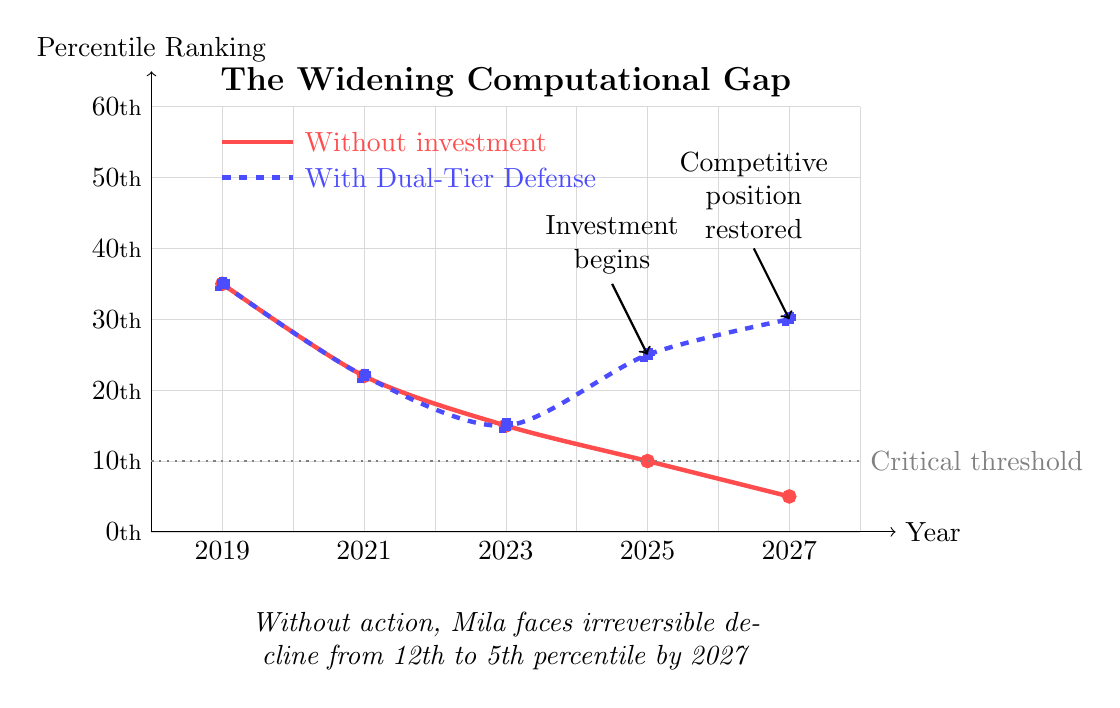
\begin{tikzpicture}[scale=0.9]
% Grid
\draw[very thin,gray!30] (0,0) grid (10,6);

% Axes
\draw[->] (0,0) -- (10.5,0) node[right] {Year};
\draw[->] (0,0) -- (0,6.5) node[above] {Percentile Ranking};

% Y-axis labels
\foreach \y/\ytext in {0/0, 1/10, 2/20, 3/30, 4/40, 5/50, 6/60}
    \draw (0,\y) node[left] {\ytext\footnotesize{th}};

% X-axis labels
\foreach \x/\xtext in {1/2019, 3/2021, 5/2023, 7/2025, 9/2027}
    \draw (\x,0) node[below] {\xtext};

% Data points and lines
% Current trajectory (declining)
\draw[ultra thick,red!70,mark=*] plot[smooth] coordinates {
    (1,3.5)  % 35th percentile in 2019
    (3,2.2)  % 22nd percentile in 2021
    (5,1.5)  % 15th percentile in 2023
    (7,1.0)  % 10th percentile in 2025
    (9,0.5)  % 5th percentile in 2027
};

% With investment trajectory (recovery)
\draw[ultra thick,blue!70,mark=square*,dashed] plot[smooth] coordinates {
    (1,3.5)  % 35th percentile in 2019
    (3,2.2)  % 22nd percentile in 2021
    (5,1.5)  % 15th percentile in 2023
    (7,2.5)  % 25th percentile in 2025
    (9,3.0)  % 30th percentile in 2027
};

% Annotations
\draw[<-,thick] (7,2.5) -- (6.5,3.5) node[above,align=center] {Investment\\begins};
\draw[<-,thick] (9,3.0) -- (8.5,4) node[above,align=center] {Competitive\\position\\restored};

% Legend
\draw[ultra thick,red!70] (1,5.5) -- (2,5.5) node[right] {Without investment};
\draw[ultra thick,blue!70,dashed] (1,5) -- (2,5) node[right] {With Dual-Tier Defense};

% Critical threshold line
\draw[dotted,thick,gray] (0,1) -- (10,1) node[right] {Critical threshold};

% Title
\node[above] at (5,6) {\large\textbf{The Widening Computational Gap}};

% Key message
\node[below,text width=8cm,align=center] at (5,-1) {
    \textit{Without action, Mila faces irreversible decline from 12th to 5th percentile by 2027}
};

\end{tikzpicture}
\caption{Projected institutional ranking decline without strategic compute investment, showing recovery potential with the Dual-Tier Defense Framework}
\label{fig:gap_visualization}
\end{figure}
